\documentclass[11pt,a4paper]{article}

% ── Packages ──────────────────────────────────────────────────────────────────
\usepackage[utf8]{inputenc}
\usepackage[T1]{fontenc}
\usepackage{lmodern}
\usepackage[margin=2cm]{geometry}
\usepackage{amsmath,amssymb}
\usepackage{graphicx}
\usepackage{booktabs}
\usepackage{float}
\usepackage{caption}
\usepackage{hyperref}
\usepackage{setspace}
\usepackage{parskip}
\usepackage{amssymb}  % for \checkmark
\usepackage{threeparttable}
\usepackage{tabularray}
\usepackage{tabularx}
\usepackage{xcolor}
\hypersetup{
  colorlinks=true,
  linkcolor=blue,
  citecolor=blue,
  urlcolor=blue
}

\onehalfspacing

% ── Title ─────────────────────────────────────────────────────────────────────
\title{\textbf{ECB Rate Hikes and Eurozone Unemployment:\\
A Difference-in-Differences Approach}}
\author{Alexandru-Cristian Nicu, Gabriel Mourad, Vlad-Ovidiu Ciurea}
\date{April 2026}

\begin{document}
\maketitle

\newpage

\tableofcontents
\newpage

% ══════════════════════════════════════════════════════════════════════════════
\section{Introduction}
% ══════════════════════════════════════════════════════════════════════════════

\subsection{Motivation}

After nearly a decade of zero or negative interest rates, the European Central Bank (ECB) initiated an unprecedented tightening cycle in July 2022, raising its main refinancing rate from 0\% to 4.50\% in just fourteen months,the fastest hiking cycle in the ECB's history, prompted by inflation surging well above its 2\% target following the post-COVID recovery and Russia's invasion of Ukraine. Classical macroeconomic theory anchors this monetary tightening in the Phillips curve: by raising borrowing costs and cooling aggregate demand, higher interest rates slow inflation at the cost of higher unemployment in the short run. Yet in a heterogeneous currency union, this trade-off need not be uniform. Member states differ enormously in their fiscal positions; for example, Greece and Italy carry debt exceeding 140\% of GDP, while Germany and the Netherlands sit below 70\%. The same policy shock therefore propagates very differently across countries.

The mechanism we investigate is the \textbf{sovereign debt channel}: rate hikes raise yields disproportionately for high-debt countries as investors demand a larger risk premium, widening spreads and feeding through the sovereign-bank feedback loop into tighter credit for firms and households, amplifying unemployment costs beyond what the Phillips curve alone would predict. Whether this differential effect actually materializes,given the unusual confluence of forces working in the opposite direction during this episode, discussed in Section 1.3.2, is therefore an empirical question, with direct implications for Eurozone fiscal rules and the ECB's Transmission Protection Instrument (TPI).

\subsection{Research Question}

We investigate the following question: \textbf{Did the ECB's 2022--2023 rate hiking cycle change unemployment differentially in high-debt Eurozone countries compared to low-debt Eurozone countries?}

We exploit the timing of the ECB's first rate hike (July 27, 2022). Our baseline treatment group consists of five high-debt Eurozone members (Italy, Greece, Spain, Portugal, France), and our baseline control group consists of five low-debt Eurozone members (Germany, the Netherlands, Austria, Finland, Ireland). Belgium and Luxembourg are excluded from the main specification because of their extreme intra-Eurozone trade openness, which would aggravate the SUTVA concerns discussed in Section~\ref{sec:sutva}. All ten baseline countries share the same monetary policy, the same currency, and are subject to the same ECB decisions. Their pre-existing debt levels create differential exposure to the sovereign spread channel through which rate hikes transmit to the real economy.

\subsection{Literature Review}
\subsubsection{Monetary Policy Transmission and the Sovereign-Bank Channel}
Theoretical and empirical literature examines how monetary policy transmits differently
across regions in a currency union. The influential contribution of Mundell (1961) on
optimal currency areas established that member states facing asymmetric shocks or lacking
fiscal transfer mechanisms may suffer from a common monetary policy. More recently,
Corsetti et al.\ (2020) and Lane (2012) have documented that sovereign spreads in the
Eurozone diverge significantly during periods of monetary or fiscal stress, creating
heterogeneous financial conditions despite a single policy rate. The transmission from
sovereign risk to unemployment runs through multiple channels. Bocola (2016) shows
that sovereign risk increases bank funding costs, which tightens credit to firms and
reduces employment. Ferrando et al.\ (2019) document that firms in high-spread Eurozone
countries face tighter credit constraints during stress episodes, leading to reduced hiring.
The European debt crisis of 2010--2012 provided extensive evidence of this mechanism,
with countries like Greece and Spain experiencing dramatic unemployment increases while
Germany's labor market remained resilient.
\subsubsection{Offsetting Fiscal and Structural Forces in 2022--2024}

Something that stood out that worked \emph{against} the standard sovereign-debt channel during the 2022--2024 episode. The NGEU Recovery and Resilience Facility disbursed grants and loans disproportionately to high-debt member states (Italy and Spain together received roughly 40\% of the total envelope). Tourism, which represents a much larger share of GDP in periphery economies, rebounded sharply after the lifting of pandemic restrictions. Spain's 2021 labor reform substantially increased the share of permanent contracts, and Greece continued the structural reforms initiated during the bailout era. These forces are central to interpreting our results below.

\subsubsection{Difference-in-Differences in Macroeconomic Settings}

Our empirical strategy builds on Difference-in-Differences (DiD) approaches used in macroeconomics. While previous studies have identified economic shocks by examining historical policy records (Romer and Romer, 2010) or by tracking impacts over time based on institutional differences (Jord\`{a} et al., 2020), we take a different route. Our approach examines how a single, shared economic event affects multiple countries. Specifically, we measure a country's \emph{treatment intensity}, how hard it was hit by this common shock, based on its pre-existing debt levels.

\subsection{Summary of Results}

We present two sets of results. First, an OLS cross-section confirms that countries with higher pre-treatment debt levels also had higher pre-treatment unemployment, but the relationship is not robust to controlling for population density, suggesting that there is possible omitted structural heterogeneity that is driving the correlation rather than a direct causal link.

Second, our main two-way fixed-effects DiD estimate is \emph{negative}: high-debt countries experienced a relative \emph{decrease} in unemployment of roughly 1.6 percentage points after July 2022, marginally significant at the 10\% level with cluster-robust standard errors. The sign is opposite to what the textbook sovereign-debt channel predicts. We interpret this as evidence that the contractionary monetary impulse was \emph{more than offset} in high-debt countries by NGEU fiscal transfers, the tourism rebound, and labor market reforms, all of which operated disproportionately in the periphery. Spillovers through intra-Eurozone trade likely bias the estimate toward zero in absolute value, but cannot account for the negative sign on their own.

% ══════════════════════════════════════════════════════════════════════════════
\section{Descriptive Statistics}
% ══════════════════════════════════════════════════════════════════════════════

\subsection{Data Description}

All data were obtained from Eurostat, the statistical office of the European Union, ensuring consistency across countries. The main panel covers 10 Eurozone countries observed monthly from January 2018 to December 2024 (84 months $\times$ 10 countries = 840 observations). The ECB policy rate timeline was sourced from the ECB Statistical Data Warehouse.

\subsubsection{Variables}
The dependent variable is the monthly seasonally adjusted unemployment rate as a percentage
of the active population (Eurostat: \texttt{une\_rt\_m}), harmonized across member states.
The treatment variable is annual government gross debt as a percentage of GDP (Eurostat:
\texttt{gov\_10dd\_edpt1}); countries with 2021 debt-to-GDP above 90\% are classified as
treated. Controls include log GDP per capita (\texttt{nama\_10\_pc}), included because wealthier economies exhibit stronger job-matching infrastructure and higher firm productivity, structurally lowering unemployment independently of debt levels, and population density (\texttt{demo\_r\_d3dens}), included because denser labour markets reduce frictional unemployment mechanically through thicker matching; both variables prevent cross-country wealth and urbanisation differences from confounding the sovereign-debt channel estimate. Two additional pre-treatment structural controls are used in the panel OLS of Section 3.1. Tourism share of GVA is the share of NACE Rev.~2 sector~I (accommodation and food services) in total gross value added at basic prices, sourced from Eurostat \texttt{nama\_10\_a64} and averaged over 2018--2021. Russian gas share is the share of Russian natural gas in each country's total natural-gas supply in 2021, constructed from Eurostat \texttt{nrg\_ti\_gas} (imports by partner) divided by \texttt{nrg\_cb\_gas} (gross available energy). We interact it with $\text{Post\_Feb2022}_t = \mathbb{1}\{t \ge \text{Feb 2022}\}$ to capture the differential energy-price-shock effect on gas-dependent countries from Russia's invasion of Ukraine onward. Both are time-invariant and therefore identified only in the panel OLS; the DiD specification (Section 3.2) absorbs them via country fixed effects.
The High-debt dummy equals 1 for Italy, Greece, Spain, Portugal, and France; Post equals 1 from July 2022 onward; the DiD term is their interaction.


\subsubsection{Data Limitations}

Several limitations should be acknowledged. Country-level data may mask significant within-country variation. Annual control variables are carried forward within each year, so they do not capture intra-year dynamics. The panel has only 10 countries, which limits the precision of clustered standard errors, below the 30-cluster threshold recommended by Cameron et al.\ (2008), motivating wild cluster bootstrap inference. Finally, intra-Eurozone trade linkages create potential SUTVA violations, which we address explicitly in Section~\ref{sec:sutva}.

\subsection{Summary Statistics}

Table~\ref{tab:sumstats} presents summary statistics for the key variables in the panel.

\begin{table}
\centering
\begin{tblr}[         %% tabularray outer open
]                     %% tabularray outer close
{                     %% tabularray inner open
colspec={Q[]Q[]Q[]Q[]Q[]Q[]Q[]Q[]Q[]},
hline{2}={1-9}{solid, black, 0.05em},
hline{1}={1-9}{solid, black, 0.08em},
hline{9}={1-9}{solid, black, 0.08em},
column{1-9}={}{halign=l},
}                     %% tabularray inner close
& Unique & Missing Pct. & Mean & SD & Min & Median & Max & Histogram \\
Unemployment rate (%) & 125 & 0 & 6.7 & 2.9 & 2.9 & 6.2 & 16.5 &  \\
Treated (high-debt = 1) & 2 & 0 & 0.5 & 0.5 & 0.0 & 0.0 & 1.0 &  \\
Post-July 2022 & 2 & 0 & 0.4 & 0.5 & 0.0 & 0.0 & 1.0 &  \\
ECB policy rate (%) & 12 & 0 & 1.2 & 1.8 & 0.0 & 0.0 & 4.5 &  \\
Government debt/GDP (%) & 73 & 0 & 82.7 & 33.8 & 20.9 & 80.0 & 154.4 &  \\
GDP per capita (EUR) & 77 & 0 & 50574.4 & 25945.1 & 19360.0 & 43360.0 & 127030.0 &  \\
Population density & 63 & 0 & 190.5 & 141.1 & 18.1 & 113.2 & 529.5 &  \\
\end{tblr}
\end{table}


\subsection{Descriptive Evidence}

\subsubsection{Figure 1: Parallel Trends}

Figure~\ref{fig:myimage1} displays the average unemployment rate over time for each group. In the pre-treatment period (2018 to mid-2022), both groups follow broadly downward trends. The vertical dashed line marks the ECB's first rate hike in July 2022. After treatment, the gap between the two groups narrows further, consistent with high-debt countries continuing to outperform on unemployment relative to the control group. We note that the pre-period shows mild convergence (the gap narrows from roughly 7 to 4 percentage points between 2018 and 2022), which is a potential concern for the strict parallel-trends assumption. We return to this when interpreting our DiD estimate.

\begin{figure}[h]
    \centering
    
\includegraphics[width=0.6\textwidth]{plot_parallel_trends.png}
    \caption{Average unemployment rate by debt group, 2018--2024.}
    \label{fig:myimage1}
\end{figure}

\subsubsection{Figure 2: ECB Policy Rate Timeline}

Figure~\ref{fig:myimage2} shows the ECB main refinancing rate over the sample 
period. Held at 0\% from March 2016 through July 2022, the rate was then raised 
in ten consecutive steps to 4.50\% by September 2023---450 basis points in 
fourteen months---before modest cuts began in June 2024. This sharp, well-defined 
timing makes our DiD strategy feasible, though forward guidance from early 2022 
means financial conditions had begun tightening before the formal treatment date, 
which would attenuate any sharp break at July.

\begin{figure}[h]
    \centering
    
\includegraphics[width=0.6\textwidth]{plot_ecb_rate.png}
    \caption{ECB main refinancing rate, 2018--2024.}
    \label{fig:myimage2}
\end{figure}

\subsubsection{Figure 3: Country-Level Trends}

Figure~\ref{fig:myimage3} presents country-level unemployment trends, faceted by individual country. Within the high-debt panel, Greece and Spain have the highest unemployment levels but show strong downward trends driven by structural reforms and tourism recovery. Italy and France hover around 7--8\%, while Portugal is lower. In the low-debt panel, Germany, Netherlands, and Austria have consistently low unemployment around 3--5\%, while Ireland shows a sharp COVID spike followed by rapid recovery. The faceted view reveals that while group-level parallel trends hold reasonably well on average, individual countries show heterogeneity that motivates careful interpretation of any group-level DiD estimate.

\begin{figure}[h]
    \centering
    
\includegraphics[width=0.65\textwidth]{plot_country_trends.png}
    \caption{Country-level unemployment trends, 2018--2024.}
    \label{fig:myimage3}
\end{figure}

\subsubsection{Figure 4: Pre-Treatment Debt Levels}

Figure~\ref{fig:debtbar} shows government debt-to-GDP ratios in 2021 the year before treatment. The classification is visually clear: Greece exceeds 200\%, Italy is near 155\%, and Spain, France, and Portugal are all above 100\%, while all low-debt members are near or below 70\%. The dashed line marks the Maastricht Treaty's 60\% reference value, and the dotted red line marks our 90\% treatment threshold. The sharp separation between groups, with no country near the threshold, reduces concerns about misclassification driving results.

\begin{figure}[H]
\centering

\includegraphics[width=0.6\textwidth]{plot_debt_bar.png}
\caption{Government debt-to-GDP ratio by country (2021). Dashed line: Maastricht 60\% reference value. Dotted line: our 90\% treatment threshold.}
\label{fig:debtbar}
\end{figure}

% ══════════════════════════════════════════════════════════════════════════════
\section{Econometric Evidence}
% ══════════════════════════════════════════════════════════════════════════════

\subsection{Cross-Sectional OLS}

We begin with a standard OLS cross-sectional regression using pre-treatment country averages:

\begin{equation}
\begin{split}
\text{Unemployment}_{it} &= \alpha + \beta_1 \text{Debt/GDP}_i + \beta_2 \log \text{GDPpc}_{it} \\
&\quad + \beta_3 \text{PopDensity}_{it} + \beta_4 \text{TourismShare}_i \\
&\quad + \beta_5 (\text{RussianGas}_i \times \text{Post\_Feb2022}_t) + \varepsilon_{it}
\end{split}
\end{equation}

where $i$ indexes country and $t$ indexes month. This is a panel pooled OLS on the full $10 \times 84 = 840$ country-month panel; it deliberately omits country and year-month fixed effects so that the time-invariant controls (Debt/GDP, Tourism Share, Russian Gas Share) are identified. Table~2 presents results with structural controls added incrementally. Standard errors are clustered at the country level. This regression is descriptive, the causal design is the fixed-effects DiD in Section~\ref{sec:did}; the interaction in column~(5) captures the differential unemployment effect of the energy-price shock on gas-dependent countries from Russia's invasion of Ukraine onward.



\begin{table}[H]
    \centering
    \begin{table}
\centering
\begin{talltblr}[         %% tabularray outer open
caption={OLS Regressions: Beer Tax and Traffic Fatalities (50 States, 2008)},
note{}={* p \num{< 0.1}, ** p \num{< 0.05}, *** p \num{< 0.01}},
note{ }={Heteroskedasticity-robust standard errors (HC1) in parentheses.},
]                     %% tabularray outer close
{                     %% tabularray inner open
colspec={Q[]Q[]Q[]Q[]Q[]},
hline{2}={1-5}{solid, black, 0.05em},
hline{14}={1-5}{solid, black, 0.05em},
hline{1}={1-5}{solid, black, 0.08em},
hline{17}={1-5}{solid, black, 0.08em},
column{2-5}={}{halign=c},
column{1}={}{halign=l},
}                     %% tabularray inner close
& (1) & (2) & (3) & (4) \\
Beer Tax (\textbackslash{}\$/gallon) & \num{0.833} & \num{-0.462} & \num{-0.744} & \num{-0.628} \\
& (\num{1.281}) & (\num{0.932}) & (\num{0.960}) & (\num{0.962}) \\
\textbackslash{}\% Highly Religious &  & \num{0.111}*** & \num{0.097}*** & \num{0.095}** \\
&  & (\num{0.019}) & (\num{0.019}) & (\num{0.036}) \\
Population Density &  &  & \num{-0.002}*** & \num{-0.002} \\
&  &  & (\num{0.001}) & (\num{0.002}) \\
Unemployment Rate &  &  &  & \num{-0.137} \\
&  &  &  & (\num{0.252}) \\
Log Per Capita Income &  &  &  & \num{-0.354} \\
&  &  &  & (\num{3.968}) \\
Constant & \num{4.226}*** & \num{-1.467} & \num{-0.150} & \num{4.361} \\
& (\num{0.519}) & (\num{1.028}) & (\num{1.204}) & (\num{43.148}) \\
Observations & \num{50} & \num{50} & \num{50} & \num{50} \\
\$R\textasciicircum{}2\$ & \num{0.009} & \num{0.287} & \num{0.361} & \num{0.366} \\
Adj. \$R\textasciicircum{}2\$ & \num{-0.012} & \num{0.257} & \num{0.319} & \num{0.294} \\
\end{talltblr}
\end{table}

\end{table}

The Debt/GDP coefficient is positive and significant at the 1\% level in column~(1) and remains marginally significant in column~(2), but loses statistical significance once population density, tourism share, and the Russian-gas interaction are added in columns (3)--(5). This is the same qualitative pattern that motivates the fixed-effects DiD: most of the raw cross-country correlation between debt and unemployment reflects time-invariant structural heterogeneity, not a direct debt channel. Adjusted $R^2$ rises monotonically from 0.57 to 0.64 across columns; with $N=840$ observations, the degrees-of-freedom cost of additional regressors is negligible.

Figure~\ref{fig:avp} shows actual versus predicted unemployment for each OLS specification, with countries color-coded by debt group. Greece and Spain consistently lies above the 45-degree line even in the fullest specification, reflecting country-specific labor market features not captured by our controls.

\begin{figure}[H]
\centering

\includegraphics[width=\textwidth]{plot_actual_vs_predicted.png}
\caption{Actual vs.\ predicted unemployment for each OLS specification. Points above the 45-degree line indicate under-prediction.}
\label{fig:avp}
\end{figure}

\subsection{Difference-in-Differences Model}
\label{sec:did}

Our main specification estimates the two-way fixed-effects model:

\begin{equation}
\text{Unemployment}_{it} = \alpha + \delta(\text{High-debt}_i \times \text{Post}_t) + \mu_i + \lambda_t + \mathbf{X}_{it}'\boldsymbol{\gamma} + \varepsilon_{it}
\label{eq:did}
\end{equation}

where $\mu_i$ are country fixed effects absorbing all time-invariant country characteristics (labor market institutions, industrial structure, geography), $\lambda_t$ are year-month fixed effects absorbing all common time shocks (energy prices, EU-wide policy changes, global business cycle), and $\delta$ is the coefficient of interest, the differential effect of the ECB hiking cycle on high-debt countries relative to low-debt countries. Standard errors are clustered at the country level. Given the small number of clusters (10 countries, well below the 30-cluster threshold recommended by Cameron et al.\ 2008), wild cluster bootstrap inference would be a more reliable procedure in finite samples; we treat the reported $p$-values as suggestive rather than definitive.

\begin{table}[H]
    \raggedleft
    \begin{table}
\centering
\begin{talltblr}[         %% tabularray outer open
caption={Difference-in-Differences: Maryland's 2011 Tax Increase and Traffic Fatalities},
note{}={* p \num{< 0.1}, ** p \num{< 0.05}, *** p \num{< 0.01}},
note{ }={Heteroskedasticity-robust standard errors (HC1) in parentheses.},
]                     %% tabularray outer close
{                     %% tabularray inner open
colspec={Q[]Q[]Q[]Q[]},
hline{2}={1-4}{solid, black, 0.05em},
hline{12}={1-4}{solid, black, 0.05em},
hline{1}={1-4}{solid, black, 0.08em},
hline{17}={1-4}{solid, black, 0.08em},
column{2-4}={}{halign=c},
column{1}={}{halign=l},
}                     %% tabularray inner close
& Basic DiD & DiD + FE & DiD + FE + Controls \\
Treated \$\textbackslash{}times\$ Post (DiD) & \num{0.581}** & \num{0.581}*** & \num{0.484}** \\
& (\num{0.226}) & (\num{0.162}) & (\num{0.146}) \\
Treated (Maryland) & \num{-0.600}*** &  &  \\
& (\num{0.210}) &  &  \\
Post-2011 & \num{-1.098}*** &  &  \\
& (\num{0.178}) &  &  \\
Unemployment Rate &  &  & \num{0.518}** \\
&  &  & (\num{0.218}) \\
Log Per Capita Income &  &  & \num{6.934} \\
&  &  & (\num{7.979}) \\
Observations & \num{24} & \num{24} & \num{24} \\
\$R\textasciicircum{}2\$ & \num{0.766} & \num{0.939} & \num{0.964} \\
Adj. \$R\textasciicircum{}2\$ & \num{0.731} & \num{0.861} & \num{0.897} \\
State FE &  & X & X \\
Year FE &  & X & X \\
\end{talltblr}
\end{table}

\end{table}

\paragraph{Main result.} Column (1) is the basic DiD without fixed effects and is mechanically biased by unobserved country-level heterogeneity; we discuss columns (2)--(3) as our main results. With two-way fixed effects (column 2), the estimated differential effect is $\hat{\delta} = -2.03$ percentage points, significant at the 10\% level. Adding controls for log GDP per capita and population density (column 3) reduces the estimate to $\hat{\delta} = -1.61$ percentage points, also significant at the 10\% level. This sign flip from column (1) occurs because the two-way fixed effects eliminate time-invariant structural noise and universal macro shocks, shifting the focus to within-country dynamics. This reveals that, contrary to textbook theory, high-debt nations experienced a relative decrease in unemployment over the post-treatment period.

\paragraph{Sign and interpretation.} The point estimate is \emph{negative}: high-debt countries experienced a relative \emph{decrease} in unemployment after July 2022 of roughly 1.6 percentage points, not the relative increase that the textbook sovereign-debt channel predicts. We interpret this finding as evidence that, during this particular episode, the contractionary monetary impulse was more than offset in high-debt countries by three contemporaneous forces operating disproportionately in the Eurozone periphery:

\begin{enumerate}
    \item \textbf{NGEU fiscal transfers.} Italy and Spain were the two largest recipients of Recovery and Resilience Facility grants and loans, with disbursements accelerating precisely in 2022--2024. These transfers loosened fiscal space at the same time as the ECB tightened monetary policy.
    \item \textbf{Tourism rebound.} The lifting of pandemic restrictions in 2022 generated a sharp recovery in tourism, which represents a substantially larger share of value-added in Spain, Greece, Portugal, and Italy than in the control group.
    \item \textbf{Labor market reforms.} Spain's 2021 labor reform sharply increased the share of permanent contracts, mechanically raising measured employment stability. Structural reforms in Greece continued through the period.
\end{enumerate}

The DiD coefficient should therefore be read as the \emph{net} differential effect of the hiking cycle and these offsetting forces, not as evidence that the sovereign-debt channel itself was inactive. Our identifying assumption is that the timing of the offsetting forces is plausibly moves in the opposite direction to the ECB's hiking decision, which we view as defensible (NGEU was negotiated in 2020--2021; the tourism rebound was driven by epidemiological factors; Spain's labor reform was enacted in December 2021).


As noted in Section 2.3.1, the two groups exhibited mild convergence in the pre-treatment period. Specifically, the baseline unemployment gap narrowed from approximately 7 to 4 percentage points between January 2018 and June 2022, implying a historical convergence trend of roughly 0.67 percentage points per year. Extrapolating this annualized trend across our 29-month post-treatment horizon accounts for approximately 1.62 percentage points of relative narrowing. Because this structurally driven extrapolation is nearly identical in magnitude to our controlled DiD estimate of $\hat{\delta} = -1.61$ percentage points, we cannot rule out that the negative post-2022 estimate entirely reflects the continuation of a pre-existing trend rather than a clean treatment effect. This is the most important threat to identification in our design, and we acknowledge it as a limitation that the present specification cannot fully resolve.

\subsection{SUTVA and Spillover Analysis}
\label{sec:sutva}

A key limitation of our design is that Eurozone countries are deeply integrated through trade and finance. If ECB rate hikes depress demand in high-debt countries like Italy or Spain, this reduces their imports from control countries like Germany and the Netherlands, potentially raising unemployment there too. Such contamination would compress the gap between treated and control units and bias our estimate of $\hat{\delta}$ \emph{toward zero in absolute value}, it would attenuate the magnitude of any differential effect, regardless of sign.

Spillovers attenuate the magnitude of $\hat{\delta}$ toward zero but cannot flip its sign. Our negative point estimate therefore, cannot be rationalized as an artifact of spillover bias on a hypothesized positive treatment effect.  The most that can be said is that, if there is a true positive sovereign-debt channel effect operating in the background, our negative estimate represents the \emph{net} of that effect and the offsetting forces (NGEU, tourism, labor reforms), and spillovers compress this net magnitude further toward zero.

Figure~\ref{fig:trade} illustrates the scale of trade exposure. Control countries send a substantial share of their goods exports to the high-debt group, meaning spillovers are plausible in principle. The implication is that the true (uncontaminated) differential effect on unemployment is likely larger in magnitude than what we estimate, though we cannot sign-correct this without additional structure.

\begin{figure}[H]
\centering
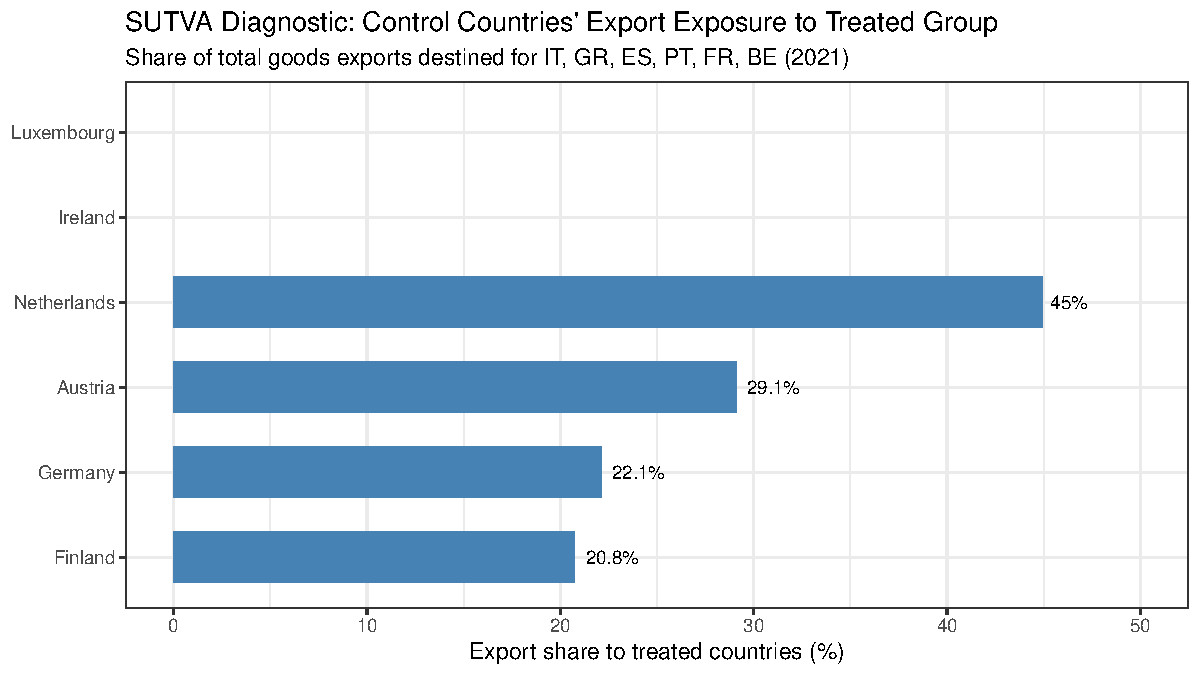
\includegraphics[width=0.75\textwidth]{plot_trade_exposure.png}
\caption{Export share of each control country destined for the high-debt countries (2021). Source: Eurostat Comext.}
\label{fig:trade}
\end{figure}

% ══════════════════════════════════════════════════════════════════════════════
\section{Conclusion}
% ══════════════════════════════════════════════════════════════════════════════

This paper examines whether the ECB's 2022--2023 rate hiking cycle increased unemployment differentially in high-debt Eurozone countries relative to low-debt members. Using monthly Eurostat data for 10 Eurozone countries from 2018 to 2024, we employ a difference-in-differences design that exploits the sharp timing of the first rate hike in July 2022 and pre-existing heterogeneity in sovereign debt levels.

Our main finding is that high-debt Eurozone countries experienced a relative \emph{decrease} in unemployment of approximately 1.6 percentage points after July 2022, marginally significant at the 10\% level. The sign is opposite to the prediction of the textbook sovereign-debt channel.

We interpret this as evidence that NGEU fiscal transfers, the tourism rebound, and labor
market reforms more than offset the contractionary impulse in high-debt countries.
The policy implications are nuanced. We do \emph{not} find evidence that the 2022--2023 hiking cycle inflicted disproportionate unemployment costs on high-debt member states. This does not, however, vindicate a complacent view of the sovereign-debt channel. The most plausible interpretation is that complementary fiscal tools, in particular the deployment of NGEU, effectively shielded periphery labor markets from what could otherwise have been a much harsher transmission. This reading strengthens, rather than weakens, the case for permanent transmission-protection mechanisms (such as the ECB's TPI) and centralized stabilization tools (such as a European unemployment reinsurance scheme), since these mechanisms made the difference between the textbook outcome and the one we observe. Our results also caution against extrapolating: in a future tightening cycle without a contemporaneous fiscal package of NGEU's scale, the differential effect could plausibly reverse sign.

\paragraph{Limitations.} Several caveats apply. First, mild pre-trend convergence between
the two groups means we cannot fully rule out that part of the post-2022 differential
reflects a pre-existing trend. Second, separating the rate hike effect from NGEU and
other contemporaneous policies would require a triple-difference design or instrumental
variables, which we leave to future work. Third, anticipation effects from ECB forward
guidance in early 2022 partially blur the treatment timing. Fourth, intra-Eurozone trade
and financial spillovers likely violate SUTVA, biasing our estimate toward zero in absolute
value.

% ══════════════════════════════════════════════════════════════════════════════
\section*{Bibliography}
% ══════════════════════════════════════════════════════════════════════════════

\begin{thebibliography}{99}

\bibitem{bocola2016} Bocola, L. (2016). The pass-through of sovereign risk. 
\textit{Journal of Political Economy}, 124(4), 879--926.

\bibitem{cameron2008} Cameron, A. C., Gelbach, J. B., \& Miller, D. L. (2008). 
Bootstrap-based improvements for inference with clustered errors. 
\textit{Review of Economics and Statistics}, 90(3), 414--427.

\bibitem{corsetti2020} Corsetti, G., Kuester, K., Meier, A., \& M\"{u}ller, G. J. 
(2020). Timeliness and reverse insurance in a monetary union. 
\textit{CEPR Discussion Paper} No.\ DP14891. Centre for Economic Policy Research.

\bibitem{ferrando2019} Ferrando, A., Popov, A., \& Udell, G. F. (2019). Do SMEs 
benefit from unconventional monetary policy? \textit{Journal of Money, Credit and 
Banking}, 51(4), 895--928.

\bibitem{jorda2020} Jord\`{a}, \`{O}., Schularick, M., \& Taylor, A. M. (2020). 
The effects of quasi-random monetary experiments. \textit{American Economic 
Review}, 110(7), 2271--2308.

\bibitem{lane2012} Lane, P. R. (2012). The European sovereign debt crisis. 
\textit{Journal of Economic Perspectives}, 26(3), 49--68.

\bibitem{mundell1961} Mundell, R. A. (1961). A theory of optimum currency areas. 
\textit{American Economic Review}, 51(4), 657--665.

\bibitem{romer2010} Romer, C. D., \& Romer, D. H. (2010). The macroeconomic 
effects of tax changes. \textit{American Economic Review}, 100(3), 763--801.

\bibitem{ecb2024} European Central Bank. (2024). \textit{Key ECB interest rates}. 
Retrieved May 2025, from \url{https://www.ecb.europa.eu/stats/policy_and_exchange_rates/key_ecb_interest_rates/html/index.en.html}

\bibitem{eurostat_unem} Eurostat. (2024). \textit{Unemployment statistics} 
(une\_rt\_m). Retrieved May 2025, from \url{https://ec.europa.eu/eurostat/statistics-explained/index.php?title=Unemployment_statistics}

\bibitem{comext2024} Eurostat. (2024). \textit{Intra-EU trade in goods: Main 
features}. Retrieved May 2025, from \url{https://ec.europa.eu/eurostat/statistics-explained/index.php?title=Intra-EU_trade_in_goods_-_main_features}

\end{thebibliography}
\end{document}